\section{Prototype One}
\begin{figure}[h!]
    \centering
    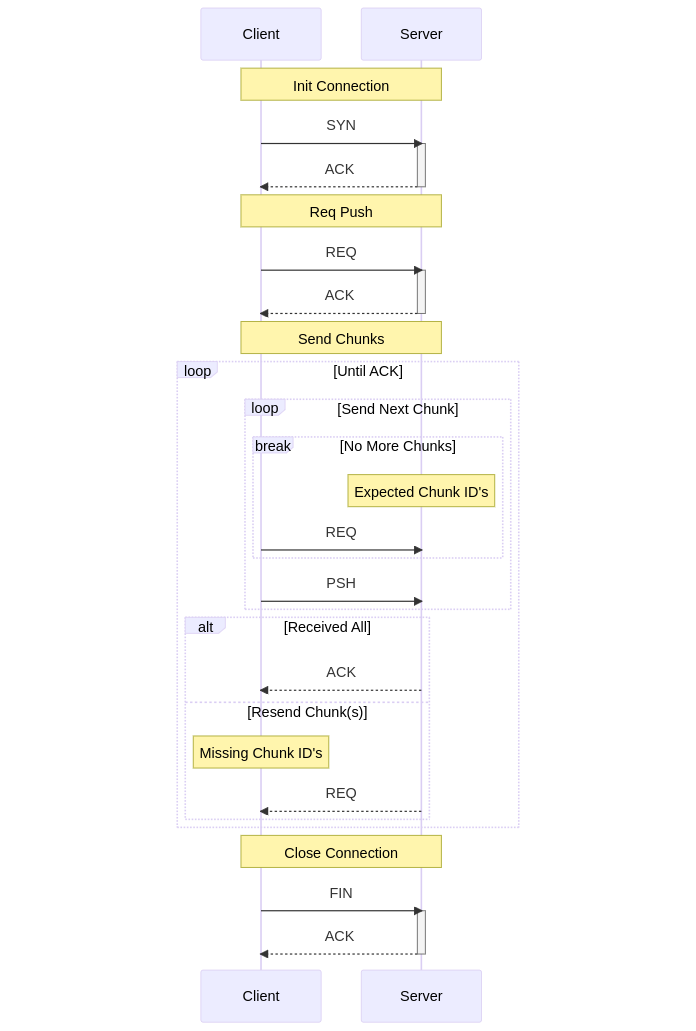
\includegraphics[width=0.8\linewidth]{p1-sequence.png}
    \caption{Prototype One Sequence Diagram}
    \label{fig:p1-sequence}
\end{figure}

\begin{table}[h!]
	\caption{Prototype One Packet Fields}
	\label{tab:p1d-packet-fields}
	\centering
	\begin{tabular}{ l l l }
		\hline
		\textbf{Num} & \textbf{Name}   & \textbf{Data-Type} \\
		\hline
		001          & Type            & uint8              \\
		\hline
		002          & Header Length   & uint64             \\
		\hline
		003          & Header          & protobuf           \\
		\hline
		004          & Metadata Length & uint64             \\
		\hline
		005          & Metadata        & protobuf           \\
		\hline
		006          & Payload Length  & uint64             \\
		\hline
		007          & Payload         & binary             \\
		\hline
	\end{tabular}
\end{table}

\begin{table}[h!]
	\caption{Prototype One Packet Types}
	\label{tab:p1d-packet-types}
	\centering
	\begin{tabular}{ l l l }
		\hline
		\textbf{Prefix} & \textbf{Value} & \textbf{Note}                \\
		\hline
		SYN             & 1              & Perform connection handshake \\
		\hline
		ACK             & 2              & Acknowledge request          \\
		\hline
		REQ             & 3              & Request to send/receive      \\
		\hline
		PSH             & 4              & Send payload data            \\
		\hline
		FIN             & 254            & End connection               \\
		\hline
	\end{tabular}
\end{table}

\begin{lstlisting}[float,caption={Prototype One Example Packet Structure},label=lst:p1d-example-structure]
|-------------------|
| 1                 | <- Packet Type
| 5                 | <- Header Length
| {id: 1, mtu: 470} | <- Protobuf Header (JSON representation)
| 0                 | <- No Metadata
| 0                 | <- No Payload
|-------------------|
\end{lstlisting}

\begin{lstlisting}[float,caption={Prototype One Example Packet Binary},label=lst:p1d-example-binary]
 1 0 0 0 0 0 0 0 5 8 1 16 214 3 0 0 0 0 0 0 0 0 0 0 0 0 0 0 0 0
 ^ ^^^^^^^^^^^^^^^ ^^^^^^^^^^^^ ^^^^^^^^^^^^^^^ ^^^^^^^^^^^^^^^
 |        |             |              |               |
Type    Header        Header        Metadata        Payload
        Length                       Length         Length
\end{lstlisting}


\FloatBarrier


\section{Prototype Two}
\FloatBarrier
\begin{figure}[h!]
    \centering
    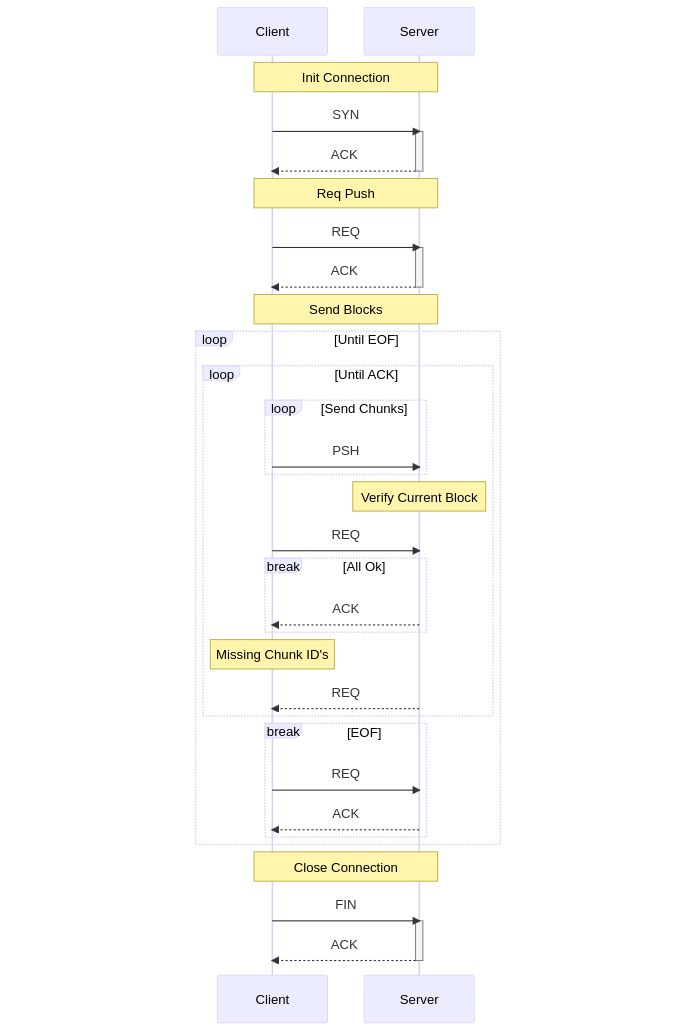
\includegraphics[width=0.8\linewidth]{p2-sequence.png}
    \caption{Prototype Two Sequence Diagram}
    \label{fig:p2-sequence}
\end{figure}

\FloatBarrier


\newpage
\section{Prototype Three}
\begin{table}[h!]
	\caption{Prototype Three Packet Fields}
	\label{tab:p3d-packet-fields}
	\centering
	\begin{tabular}{ l l l }
		\hline
		\textbf{Num} & \textbf{Name}  & \textbf{Data-Type} \\
		\hline
		001          & Type           & uint8              \\
		\hline
		002          & Header Length  & uint32             \\
		\hline
		003          & Header         & protobuf           \\
		\hline
		004          & Payload Length & uint32             \\
		\hline
		005          & Payload        & binary             \\
		\hline
	\end{tabular}
\end{table}

\begin{table}[h!]
	\caption{Prototype Three Packet Types}
	\label{tab:p3d-packet-types}
	\centering
	\begin{tabular}{ l l l }
		\hline
		\textbf{Prefix} & \textbf{Value} & \textbf{Note}                        \\
		\hline
		REQ\_SYN         & 1              & Start connection, share capabilities \\
		\hline
		REQ\_FIN         & 2              & Finalise connection                  \\
		\hline
		REQ\_PSH         & 10             & Request to send a file               \\
		\hline
		REQ\_PSH\_DAT     & 11             & Chunk of file data                   \\
		\hline
		REQ\_PSH\_VAL     & 12             & Request to validate current block    \\
		\hline
		REQ\_PSH\_EOF     & 13             & Mark EOF, transfer finished          \\
		\hline
		RES\_SYN         & 1              & Reply to REQ\_SYN, share capabilities \\
		\hline
		RES\_ACK         & 2              & Acknowledge REQ\_*                    \\
		\hline
		RES\_ERR\_DAT     & 10             & Chunk ID's to re-send                \\
		\hline
	\end{tabular}
\end{table}

\begin{lstlisting}[float,caption={Prototype Three Example Packet Structure},label=lst:p3d-example-structure]
|-------------------|
| 1                 | <- Packet Type
| 5                 | <- Header Length
| {id: 1, mtu: 470} | <- Protobuf Header (JSON representation)
| 0                 | <- Payload Length (No Payload)
|-------------------|
\end{lstlisting}

\begin{lstlisting}[float,caption={Prototype Three Example Packet Binary},label=lst:p3d-example-binary]
 1    0 0 0 5    8 1 16 214 3    0 0 0 0
 ^    ^^^^^^^    ^^^^^^^^^^^^
 |       |            |            |
Type   Header       Header       Payload
       Length                    Length
\end{lstlisting}
